\documentclass[a4j,twoside,openright,11pt]{jreport}
%
\usepackage{amsmath,amssymb}
\usepackage{bm}
\usepackage{graphicx}
\usepackage{ascmac}
\usepackage{listliketab}
\usepackage{url}
\usepackage{listings}

\setlength{\textwidth}{15.92cm}
\setlength{\oddsidemargin}{0mm}
\setlength{\evensidemargin}{0mm}
\setlength{\topmargin}{-1cm}
\setlength{\textheight}{23.5cm}
\setlength{\footskip}{18mm}

%
\pagestyle{plain}
\title{設計製図I\hspace{-.1em}I \\計算書}
\author{九州工業大学 機械知能工学科 機械知能コース 3年\\学籍番号:13104069 坂本悠作}
\date{\today}
\begin{document}
\maketitle
\chapter{歯車設計編}
与えられたデータを以下に示す.
\begin{table}[htb]
\begin{center}
  \caption{データ}
  \begin{tabular}{|l|c|} \hline
    入力動力(kw)&17\\
    回転数(rpm)&1300\\
    速度伝達比&12\\
    ねじれ角(deg)&21\\
    \hline
  \end{tabular}
\end{center}
\end{table}
\section{手順A:歯数仮定$Z_1Z_2Z_3Z_4$ }
以下の式より,$u_1,u_2$を算出する.
\begin{eqnarray}
u_i&=&1.15 \sqrt i \approx 3.9837\nonumber\\
u_2&=&0.87 \sqrt i \approx 3.0137 \nonumber
\end{eqnarray}

ピニオン(小歯車)の歯数を仮定する.歯数の範囲は,21$\sim$25の範囲で定める\\
ここでは,以下のように仮定した.
\begin{table}[htb]
\begin{center}
  \caption{歯数の仮定}
  \begin{tabular}{|l|c|} \hline
    $Z_1$&21\\
    $Z_2$&83\\
    $Z_3$&24\\
    $Z_4$&74\\
    \hline
  \end{tabular}
\end{center}
\end{table}
\section{手順B:モジュールの選定}
モジュールの仮定は,以下のように定めた
\begin{table}[htb]
\begin{center}
  \caption{モジュールの仮定}
  \begin{tabular}{|l|c|} \hline
    歯車の組み合わせ&モジュール\\\hline
    $Z_1とZ_2$&4\\
    $Z_3とZ_4$&4.5\\
    \hline
  \end{tabular}
\end{center}
\end{table}
\section{手順C:歯幅bの仮定}
\begin{equation}
1.3\times1.25 \pi m_t /tan{\beta} \geq b \geq 1.25 \pi m_t /tan{\beta}\nonumber\\
\end{equation}
\begin{table}[htb]
\begin{center}
  \caption{bの仮定}
  \begin{tabular}{|l|c|c|c|c|} \hline
    歯車の組み合わせ&モジュール&bの値&bの最大許容値&bの最小許容範囲\\\hline
    $Z_1とZ_2$&4&41&53.197&40.920\\
    $Z_3とZ_4$&4.5&58&59.846&46.036\\
    \hline
  \end{tabular}
\end{center}
\end{table}

モジュールが決定したので,以下のものが決定される
\begin{table}[htb]
\begin{center}
  \caption{$d_{a,b}の算出[mm]$}
  \begin{tabular}{|l|c|c|c|} \hline
    歯車番号&ピッチ円筒直径(d)&歯先円直径($d_a$)&基礎円直径($d_b$)\\\hline
    1       &89.976  &97.976  &$ 83.831$\\
    2       &351.335 &359.335 &$327.338$\\
    3       &110.864 &119.864 &$103.291$\\
    4       &356.691 &365.691 &$332.328$\\
    \hline
  \end{tabular}
\end{center}
\end{table}

\section{手順D:$\sigma_F$の算出}
歯元曲げ応力の式を以下に示す.
\begin{equation}
\sigma_F=F_W/(bm\cos{\alpha_t})YY_{\epsilon}K_{\delta}K_AK_VK_{\beta}\nonumber
\end{equation}
ここで,L=17(kw),$n_1$=1300(rpm),$r_1$=44.988より,
\begin{eqnarray}
F_{W12} &=& 9.74\times10^5L/(r_1n_1)\nonumber\\
       &=& 283.117668[kgf]\nonumber\\
F_{W34} &=& 9.74\times10^5L/(r_3n_3)\nonumber\\
       &=& 897.223143[kgf]\nonumber
\end{eqnarray}

\begin{itemize}
\item $\alpha_t=0.371738799[radian]$
\item $Y=2.56$
\item $Y_{\epsilon}=1.0$
\item $K_A=1.25$
\item $K_{\delta}=1.0$
\item $K_V=1.2$
\item $K_{\beta}=1.5$
\end{itemize}
上の条件により,
\begin{eqnarray}
\sigma_{F1}&=&283.11766/(41\times4\times\cos{0.371738799}) 2.56 \times 1.0 \times 1.0 \times 1.25 \times 1.2 \times 1.5\nonumber\\
&=&10.8393741 [kgfmm]\nonumber
\end{eqnarray}

同様の計算により,以下の値が算出される.

\begin{table}[htb]
\begin{center}
  \caption{$\sigma_F$の算出[kgfmm]}
  \begin{tabular}{|l|c|c|} \hline
    歯車No.     &$\sigma_F$ &安全率$S_F$\\\hline
    1           &10.839 &2.445\\
    2           & 8.588 &2.970\\
    3           &26.226 &1.247\\
    4           &21.719 &1.477\\
    \hline
  \end{tabular}
\end{center}
\end{table}
$S_F=\frac{\sigma_{Flim}}{\sigma_{F}}...曲げ強さに対する安全係数$\\

\section{手順G:歯車材選定}
\subsection{歯車1の材料}
炭素鋼(焼入焼戻し)
\begin{itemize}
\item 硬さ$ H_B = 290,H_V=305$
\item 引っ張り強さ(下限)$912.0[N/mm^2]$
\item 曲げ強さ$\sigma_{Flim}=255.9[N/mm^2]$
\item 歯面強さ$\sigma_{Hlim}6686.5[N/mm^2]$
\end{itemize}
\subsection{歯車2の材料}
炭素鋼(焼入焼戻し)
\begin{itemize}
\item 硬さ$ H_B = 270,H_V=284$
\item 引っ張り強さ(下限)$853.2[N/mm^2]$
\item 曲げ強さ$\sigma_{Flim}=255.0[N/mm^2]$
\item 歯面強さ$\sigma_{Hlim}657.0[N/mm^2]$
\end{itemize}
\subsection{歯車3の材料}
炭素鋼(焼入焼戻し)
\begin{itemize}
\item 硬さ$ H_B = 290,H_V=305$
\item 引っ張り強さ(下限)$912.0[N/mm^2]$
\item 曲げ強さ$\sigma_{Flim}=255.9[N/mm^2]$
\item 歯面強さ$\sigma_{Hlim}6686.5[N/mm^2]$
\end{itemize}
\subsection{歯車4の材料}
炭素鋼(焼入焼戻し)
\begin{itemize}
\item 硬さ$ H_B = 270,H_V=284$
\item 引っ張り強さ(下限)$853.2[N/mm^2]$
\item 曲げ強さ$\sigma_{Flim}=255.0[N/mm^2]$
\item 歯面強さ$\sigma_{Hlim}657.0[N/mm^2]$
\end{itemize}
を仮定する.
\section{手順E:$\sigma_H$の算出}
$\sigma_H$を算出するには,以下の式を用いる.
\begin{equation}
\sigma_H=\sqrt K Z_{HH}Z_{E}\sqrt K_A \sqrt K_V \sqrt K_B\nonumber
\end{equation}
これを計算するためには,$\sqrt K, Z_{HH},Z_{E}$の値を計算する.
\begin{eqnarray}
K &=&\frac{F_W}{bd_1}\frac{u+1}{u}\nonumber\\
Z_{HH}&=&2\sqrt{cos{\beta_b}}/\sqrt{\epsilon_a \sin{2_{\alpha_i}}}\nonumber\\
Z_E&=&\sqrt{0.35E_1E_2/(E_1+E_2)}\nonumber
\end{eqnarray}

\begin{table}[htb]
\begin{center}
  \caption{$\sigma_H$の算出[kgfmm]}
  \begin{tabular}{|l|c|c|} \hline
    歯車No.&$\sigma_H[N/mm^2]$&安全率$S_H$\\\hline
    1      &469.5756  &1.4619\\
    2      &469.5756  &1.3991\\
    3      &645.9699  &1.0627\\
    4      &645.9699  &1.0170\\
    \hline
  \end{tabular}
\end{center}
\end{table}
$S_H=\frac{\sigma_{Hlim}}{\sigma_{H}}...歯面強さに対する安全係数$\\
\section{手順N}
\subsection{バックラッシの計算}
汎用減速機の歯車には通常歯車精度等級に$3\sim 4$級が使用される.よって,ここでは3級として計算をしていく.バックラッシの計算は,次式で求まる.
\begin{eqnarray}
最大値 j_{t(max)}&=&35.5 \omega  [\mu m]\nonumber\\
最小値 j_{t(min)}&=&10 \omega  [\mu m]\nonumber\\
ただしここでは, \omega &=& d^{1/3} + 0.65 m_t\nonumber
\end{eqnarray}
この計算式によって計算すると,次の計算結果が算出される.
\begin{table}[htb]
\begin{center}
  \caption{バックラッシの計算結果}
  \begin{tabular}{|l||c|c|c|c|c|} \hline
歯車番号&最大値($\mu m$)&最小値($\mu m$)&$\omega$&合計値(max)&合計値(min)\\\hline
1&257.943& 72.660& 7.266&171.072	&607.306\\
2&349.364& 98.412& 9.841&&\\
3&281.764& 79.370& 7.937&181.620	&644.753\\
4&362.988&102.250&10.225&&\\
\hline
  \end{tabular}
\end{center}
\end{table}

\subsection{中心間距離寸法公差の計算}
中心距離寸法公差等級はH7として計算する.H7の中心距離寸法公差は以下のとおりである.
\begin{equation}
\Delta a=16 \omega_c
\end{equation}
ここで,$\omega_c = 0.45a^{1/4}+0.001a (a:中心距離)$である.
\begin{table}[htb]
\begin{center}
  \caption{中心間距離寸法公差の計算結果}
  \begin{tabular}{|l||c|c|} \hline
段 &$\omega_c(\mu m)$&$\Delta a(\mu m)$\\\hline
12(1段目)&2.940&47.039\\
34(2段目)&3.006&48.094\\
\hline
  \end{tabular}
\end{center}
\end{table}

\subsection{歯厚寸法差}
次に示すのは,歯厚寸法差$\Delta s(\mu m)$の計算式である.
\begin{equation}
\Delta s_1 = \Delta s_2 =(-j_t + 2\Delta a \tan \alpha_n)/2 \nonumber
\end{equation}
$\Delta s$はバックラッシと中心距離寸法公差の組み合わせで最大,最小の値を計算すると,次のようになる.
\begin{table}[htb]
\begin{center}
  \caption{歯厚の寸法差の計算結果}
  \begin{tabular}{|l||c|c|} \hline
段    &$\Delta s_{max}(\mu m)$	&$\Delta s_{min}(\mu m)$\\\hline
12    &-153.951	&-590.185\\
34    &-164.115	&-627.248\\\hline
  \end{tabular}
\end{center}
\end{table}

\subsection{またぎ歯厚}
またぎ歯厚W(mm)は次式で計算する.
\begin{eqnarray}
またぐ歯数 Z_m &=& Z(\alpha_t/180 + \tan \alpha_t \tan^2 \beta_b/\pi) + 0.5 (最も近い整数値)\\
inv(\alpha_t) &=& \tan \alpha_t - \alpha_t\\
W &=& m\cos \alpha_n(\pi (Z_m - 0.5) + Zinv(\alpha_t)) - | \Delta s |\cos \alpha_n \cos \beta
\end{eqnarray}
\begin{table}[htb]
\begin{center}
  \caption{またぎ歯厚計算結果}
  \begin{tabular}{|l||c|c|c|c|c|} \hline
歯車番号&Z&Zm&m&W(max)[mm]&W(min)[mm]\\\hline
1&21&3 &  4&34.575 & 34.192\\
2&83&12&  4&136.669&137.052\\
3&24&4 &4.5& 44.483& 44.077\\
4&74&10&4.5&137.456&137.050\\
\hline
  \end{tabular}
\end{center}
\end{table}

\section{簡易平面図}
\begin{figure}[htbp]
\begin{center}
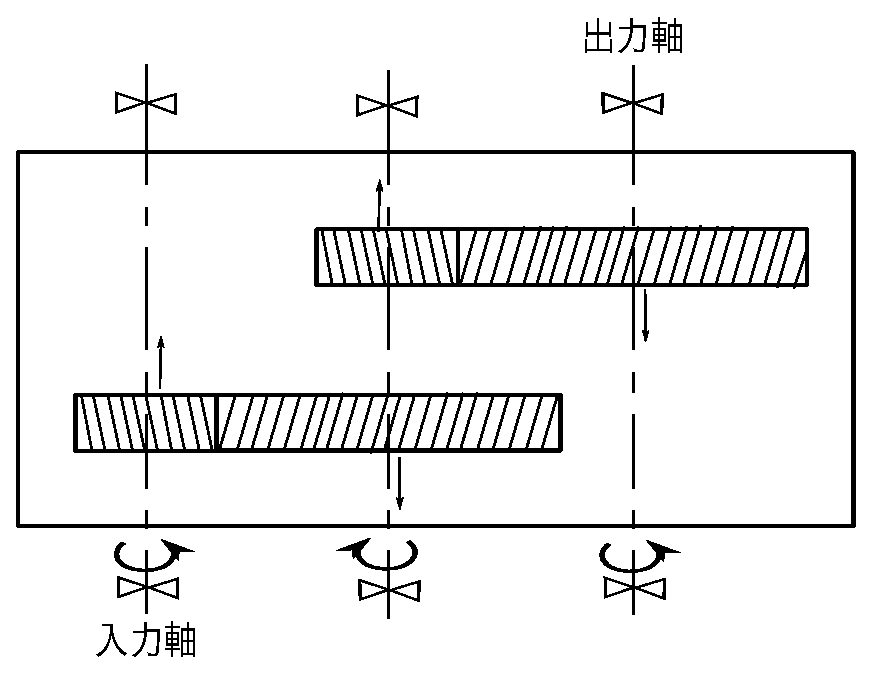
\includegraphics[width=12cm]{hagu.eps}
\end{center}
\caption{簡易平面図}
\end{figure}

\chapter{軸設計書}
\section{歯車周速}
ピッチ円周上における歯車の速度を以下のようにして求めた.
\begin{eqnarray}
v_{12}=\frac{\pi d_1 n_1}{1000} \times \frac{1}{60} = \frac{\pi \times 98.5453 \times 1300}{1000} \times \frac{1}{60} = 6.7077 [m/s]\\
v_{34}=\frac{\pi d_3 n_3}{1000} \times \frac{1}{60} = \frac{\pi \times 128.537 \times 328.5714}{1000} \times \frac{1}{60} = 2.2113 [m/s]
\end{eqnarray}

\section{動力と接線力の関係}
動力と接線力には次の関係が有る.
\begin{eqnarray}
T[N \cdot m]=F[N] r[m]\\
P[kW] = \frac{2\pi T[N \cdot m] n[rpm] }{60}w
\end{eqnarray}

以上より,接線力は以下のように算出できる.
\begin{eqnarray}
P[W] &=& \frac{\pi F[N] d[m] n[rpm] }{60}=F[N]v[N \cdot m]より,\nonumber\\
F_{12}&=& \frac{60P}{\pi d[m] n[rpm] } = \frac{60 \times 17000}{\pi \times 0.098545 \times  1300 } = 2534.4008[N]\\
F_{34}&=& \frac{60P}{\pi d[m] n[rpm] } = \frac{60 \times 17000}{\pi \times 0.128537 \times 328.5714} = 7687.6284[N]
\end{eqnarray}

\section{スラスト荷重とラジアル荷重の算出}
軸に加えられる力を,軸に対して直角に作用するラジアル荷重と,軸方向に作用するスラスト荷重に分類分けをする.こうすることでかかる力とモーメントの関係をそれぞれ算出し,後で合成することで計算ができる.\\
歯車の形状から,ラジアル荷重$P_r$とスラスト荷重$P_t$は以下のように計算される.ここに,正面圧力角(歯車を正面から見た時のピッチ円周上の歯の角度)$\alpha_t=21.2991[degree]$,ピッチ円筒ねじれ角$
\beta =21[degree]$とする\\
\begin{eqnarray}
P_r = F\tan(\alpha)\\
P_t = F\tan(\beta)
\end{eqnarray}
よって,

\begin{eqnarray}
P_{r1} &=&P_{r2} = F\tan(\alpha) = 2534.4008 \times \tan(21.2991) = 988.08[N]\\
P_{r3} &=&P_{r4} = F\tan(\alpha) = 7687.6284 \times \tan(21.2991) = 2997.14[N]\\
P_{t1} &=&P_{t2} = F\tan(\beta) = 2534.4008 \times \tan(21) = 972.87[N]\\
P_{t3} &=&P_{t4} = F\tan(\beta) = 7687.6284 \times \tan(21) = 2951[N]
\end{eqnarray}

\section{スパンの決定}
\subsection{湯浴式潤滑法}
湯浴式の潤滑法とは,歯末部分が潤滑油に浸されており,歯車の回転運動の遠心力により潤滑油が飛沫(ひまつ)して軸受けなど各部へ供給される方法である.この方法は歯車の周速が$3\sim13m/s$であるものが適している.理由としては,飛び散らせるための力として3m/s以上が好ましいということと,速すぎると潤滑油が必要以上に飛ばされるため,十分な油膜の形成に影響が出て,かつ動力損失を増してしまうため,13m/s以下が好ましいことが挙げられる.同様な理由により,ギヤボックスと歯車の間隔にも制約が入る.しかし,間隔が開きすぎると材料にかかる応力が大きくなるので,ここでは以下の式を用いて最大値と最小値を求める.ここに,Cをギヤボックスと車軸の間隔とすると,
\begin{eqnarray}
C=(2\sim3)v+10 + \alpha
\end{eqnarray}
\subsection{最大値と最小値の計算}
この式を用いて最大値と最小値を計算する
\begin{eqnarray}
C_{1max}=3v+10=3 \times 6.7077 + 10 +\alpha = 30.1231 +\alpha\\
C_{1min}=2v+10=2 \times 6.7077 + 10 +\alpha = 23.4154 +\alpha
\end{eqnarray}
\par
ここで第3歯車を固定し,相対的な速度が潤滑に影響するパラメータであると考えると,次のようになる.
\begin{eqnarray}
C_{2max}=3v+10=3 \times (6.7077-2.2113) + 10 +\alpha = 23.4892 +\alpha\\
C_{2min}=2v+10=2 \times (6.7077-2.2113) + 10 +\alpha = 18.9928 +\alpha
\end{eqnarray}
\begin{eqnarray}
C_{3max}=3v+10=3 \times 2.2113 + 10 +\alpha = 16.6339 +\alpha\\
C_{3min}=2v+10=2 \times 2.2113 + 10 +\alpha = 14.4226 +\alpha
\end{eqnarray}
\subsection{スパンの決定}
先ほどの計算から,きりのいい整数値で決定すると,
\begin{eqnarray}
C_1=24,C_2=20,C_3=15\nonumber
\end{eqnarray}
ここでギヤボックスの幅を40mmとすると,軸の長さが計算できる.
\begin{eqnarray}
軸長&=&C_1+C_2+C_3+b_{12}+b_{34}+40 \times 2\\
    &=&24+20+15+45+65+40 \times 2\\
    &=&249
\end{eqnarray}

よって,スパン長が決定する.
\begin{eqnarray}
a_1&=&\frac{40}{2} + 15 + \frac{65}{2} = 67.5\\
a_2&=&\frac{65}{2} + 20 + \frac{45}{2} = 75\\
a_3&=&\frac{45}{2} + 24 + \frac{40}{2} = 66.5
\end{eqnarray}

\section{軸に作用する力の算出}
\subsection{入力軸}
図2.1と図2.2は入力軸に作用する力をモデル化したものである.このモデルに対して,材力の公式を用いて力の分析をする.
\begin{figure}[htbp]
\begin{center}
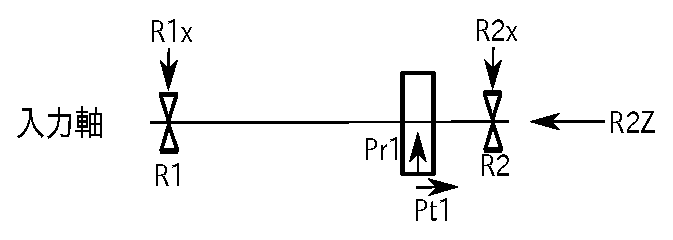
\includegraphics[width=12cm]{jiku1.eps}
\end{center}
\caption{入力軸モデル(xz成分)}
\end{figure}
\begin{figure}[htbp]
\begin{center}
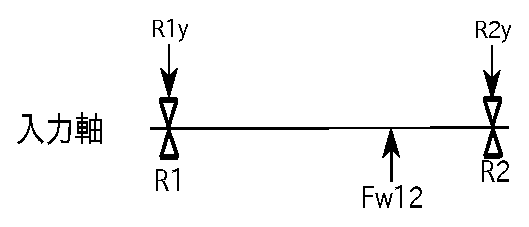
\includegraphics[width=9cm]{jiku12.eps}
\end{center}
\caption{入力軸モデル(y成分)}
\end{figure}
\subsubsection{正回転の場合}
釣り合いの式を以下に示す.
\begin{eqnarray}
x成分&:&P_{r1}-R_{1x}-R_{2x}=0\\
y成分&:&Fw_{12}-R_{1y}-R_{2y}=0\\
z成分&:&-P_{t1}+R_{2z}=0\\
y軸,R_1回りのモーメント&:&(a_1+a_2)P_{r1}+\frac{d_1}{2}P_{t1}-(a_1+a_2+a_3)R_{2x}\\
x軸,R_1回りのモーメント&:&(a_1+a_2)Fw_{12}-(a_1+a_2+a_3)R_{2y}
\end{eqnarray}
この方程式を解くことで,次の結果を得る.
\begin{itemize}
\item $R_{1x}=85.030$
\item $R_{1y}=806.401$
\item $R_{2x}=903.040$
\item $R_{2y}=1728.000$
\item $R_{2z}=972.870$
\end{itemize}
上の結果から,軸受けにかかるラジアル荷重の大きさが以下のように算出できる.
\begin{eqnarray}
R_1 &=& \sqrt {R_{1x}^2+R_{1y}^2}\\
    &=& \sqrt {85.030^2+806.401^2}=810.871\\
R_2 &=& \sqrt {R_{2x}^2+R_{2y}^2}\\
    &=& \sqrt {903.040^2+1728.000^2}=1949.735
\end{eqnarray}
次に,この軸にかかるモーメントを求め,BMDに示す.
歯車が有る点を中心に考えると,軸受けのラジアル力によって軸にかかるモーメントは次のように求めることができる.
\begin{figure}[htbp]
\begin{center}
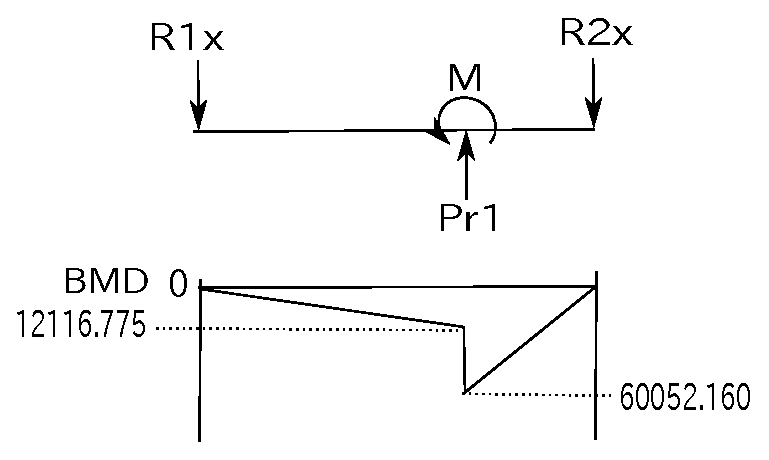
\includegraphics[width=9cm]{jiku14.eps}
\end{center}
\caption{入力軸モデル(x成分BMD)}
\end{figure}
\begin{figure}[htbp]
\begin{center}
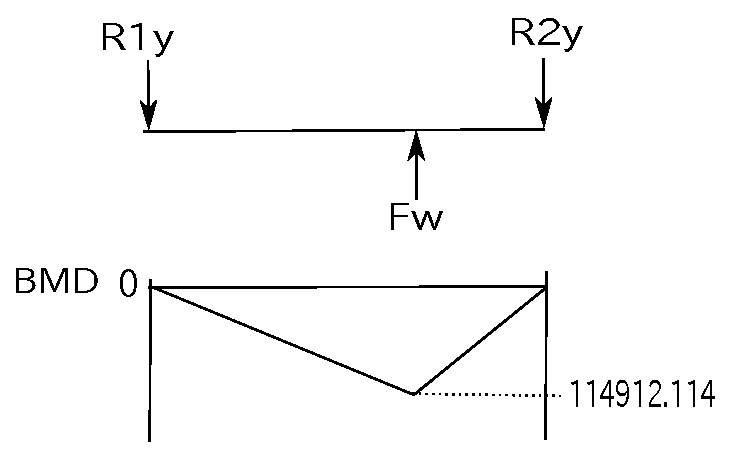
\includegraphics[width=9cm]{jiku13.eps}
\end{center}
\caption{入力軸モデル(y成分BMD)}
\end{figure}
\begin{eqnarray}
M_{1x} &=& R_{1y} \times (a_1+a_2)=114912.114\\
M_{2x} &=& R_{2y} \times a_3=114912.114\\
M_{1y} &=& R_{1x} \times (a_1+a_2)=12116.775\\
M_{2y} &=& R_{2x} \times a_3=60052.160
\end{eqnarray}
最大曲げモーメントを算出する.
\begin{eqnarray}
M_{1max} &=& \sqrt {M_{1x}^2+M_{1y}^2}\\
         &=& \sqrt {114912.114^2+12116.775^2}=115549.168\\
M_{2max} &=& \sqrt {M_{2x}^2+M_{2y}^2}\\
         &=& \sqrt {114912.114^2+60052.160^2}=129657.355
\end{eqnarray}
軸に作用するねじりモーメントを求める
\begin{eqnarray}
T_{1} &=& 0\\
T_{2} &=& \frac{d_1}{2} \times Fw_{12}\\
      &=& \frac{98.545}{2} \times 2534.4008 = 124877.531
\end{eqnarray}
軸に作用する荷重(軸力:スラスト力)を求める.
\begin{eqnarray}
T_{z1} &=& 0\\
T_{z2} &=& R_{2z} = P_{t1} = 972.870
\end{eqnarray}
\subsubsection{逆回転の場合}
釣り合いの式を以下に示す.
\begin{eqnarray}
x成分&:&P_{r1}-R_{1x}-R_{2x}=0\\
y成分&:&Fw_{12}-R_{1y}-R_{2y}=0\\
z成分&:&P_{t1}-R_{2z}=0\\
y軸,R_1回りのモーメント&:&(a_1+a_2)P_{r1}-\frac{d_1}{2}P_{t1}-(a_1+a_2+a_3)R_{2x}\\
x軸,R_1回りのモーメント&:&(a_1+a_2)Fw_{12}-(a_1+a_2+a_3)R_{2y}
\end{eqnarray}
この方程式を解くことで,次の結果を得る.
\begin{itemize}
\item $R_{1x}=543.746$
\item $R_{1y}=806.401$
\item $R_{2x}=444.324$
\item $R_{2y}=1728.000$
\item $R_{2z}=-972.870$
\end{itemize}
上の結果から,軸受けにかかるラジアル荷重の大きさが以下のように算出できる.
\begin{eqnarray}
R_1 &=& \sqrt {R_{1x}^2+R_{1y}^2}\\
    &=& \sqrt {543.746^2+806.401^2}=972.595\\
R_2 &=& \sqrt {R_{2x}^2+R_{2y}^2}\\
    &=& \sqrt {444.324^2+1728.000^2}=1784.211
\end{eqnarray}
次に,この軸にかかるモーメントを求め,BMDに示す.
歯車が有る点を中心に考えると,軸受けのラジアル力によって軸にかかるモーメントは次のように求めることができる.
\begin{figure}[htbp]
\begin{center}
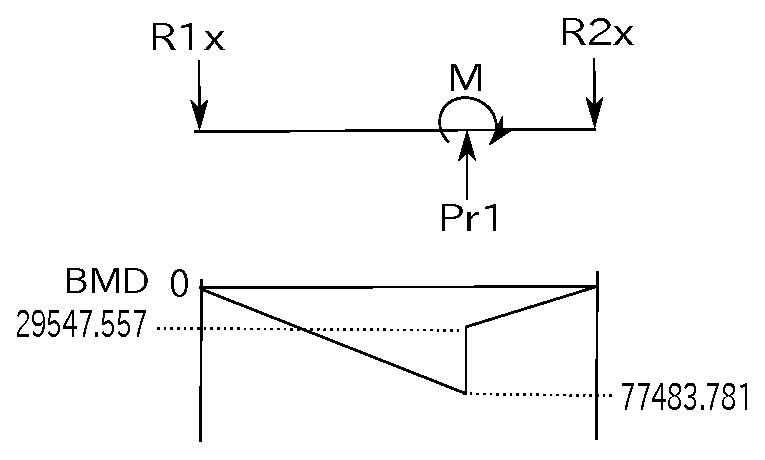
\includegraphics[width=9cm]{jiku142.eps}
\end{center}
\caption{入力軸モデル(x成分BMD)}
\end{figure}
\begin{figure}[htbp]
\begin{center}
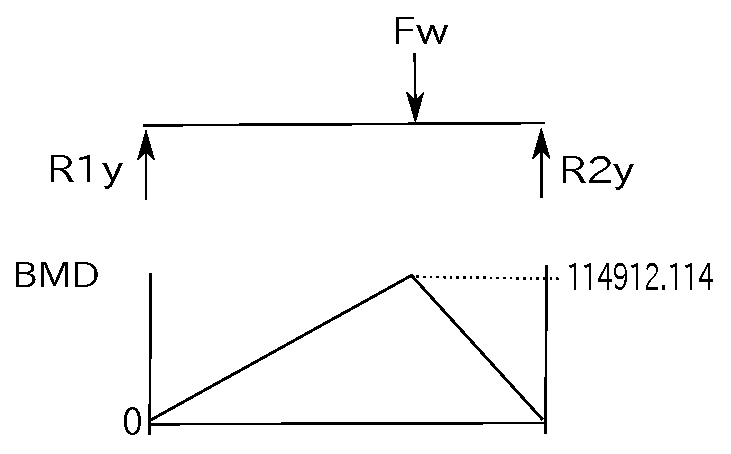
\includegraphics[width=9cm]{jiku132.eps}
\end{center}
\caption{入力軸モデル(y成分BMD)}
\end{figure}
\begin{eqnarray}
M_{1x} &=& R_{1y} \times (a_1+a_2)=114912.114\\
M_{2x} &=& R_{2y} \times a_3=114912.114\\
M_{1y} &=& R_{1x} \times (a_1+a_2)=77483.781\\
M_{2y} &=& R_{2x} \times a_3=29547.557
\end{eqnarray}
最大曲げモーメントを算出する.
\begin{eqnarray}
M_{1max} &=& \sqrt {M_{1x}^2+M_{1y}^2}\\
         &=& \sqrt {114912.114^2+77483.781^2}=138594.747\\
M_{2max} &=& \sqrt {M_{2x}^2+M_{2y}^2}\\
         &=& \sqrt {114912.114^2+29547.557^2}=118650.014
\end{eqnarray}
軸に作用するねじりモーメントを求める
\begin{eqnarray}
T_{1} &=& 0\\
T_{2} &=& \frac{d_1}{2} \times Fw_{12}\\
      &=& \frac{98.545}{2} \times 2534.4008 = 124877.531
\end{eqnarray}
軸に作用する荷重(軸力:スラスト力)を求める.
\begin{eqnarray}
T_{z1} &=& 0\\
T_{z2} &=& R_{2z} = P_{t1} = 972.870
\end{eqnarray}




\subsection{中間軸}
\subsubsection{正回転の場合}
\begin{figure}[htbp]
\begin{center}
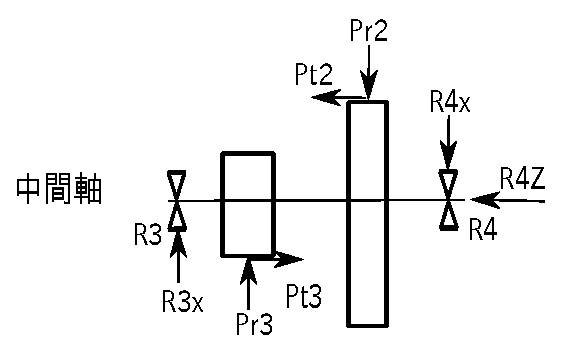
\includegraphics[width=10cm]{jiku4.eps}
\end{center}
\caption{中間軸モデル}
\end{figure}
釣り合いの式を以下に示す.
\begin{eqnarray}
x成分&:&P_{r3}-P_{r2}+R_{3x}-R_{4x}=0\\
y成分&:&-Fw_{12}-Fw_{34}+R_{3y}+R_{4y}=0\\
z成分&:&-P_{t2}+P_{t3}+R_{4z}=0\\
y軸,R_3回りのモーメント&:&a_1P_{r3}-(a_1+a_2)P_{r2}-(a_1+a_2+a_3)R_{4x}-\frac{d_3}{2}P_{t3}-\frac{d_2}{2}P_{t2}\nonumber\\
\\
x軸,R_3回りのモーメント&:&-a_1Fw_{34}-(a_1+a_2)Fw_{12}+(a_1+a_2+a_3)F_{4y}
\end{eqnarray}
この方程式を解くことで,次の結果を得る.
\begin{itemize}
\item $R_{3x} = 100.142$
\item $R_{3y} = 6011.182$
\item $R_{4x} = 2109.198$
\item $R_{4y} = 4210.847$
\item $R_{4z} = 1978.130$
\end{itemize}
上の結果から,軸受けにかかるラジアル荷重の大きさが以下のように算出できる.
\begin{eqnarray}
R_3 &=& \sqrt {R_{3x}^2+R_{3y}^2}\\
    &=& \sqrt {100.142^2+6011.182^2}=6012.016\\
R_4 &=& \sqrt {R_{4x}^2+R_{4y}^2}\\
    &=& \sqrt {2109.198^2+4210.847^2}=4709.559
\end{eqnarray}
次に,この軸にかかるモーメントを求め,BMDに示す.
歯車が有る点を中心に考えると,軸受けのラジアル力によって軸にかかるモーメントは次のように求めることができる.
\begin{figure}[htbp]
\begin{center}
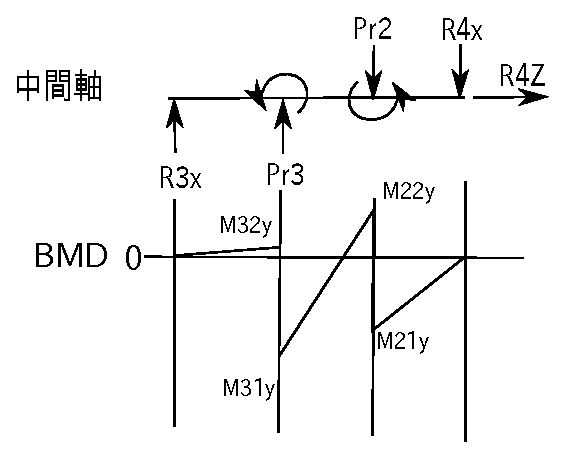
\includegraphics[width=10cm]{jiku47.eps}
\end{center}
\caption{中間軸y軸基準}
\end{figure}
\begin{figure}[htbp]
\begin{center}
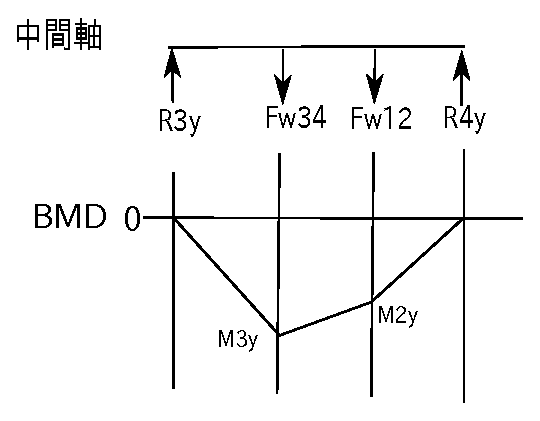
\includegraphics[width=10cm]{jiku45.eps}
\end{center}
\caption{中間軸x軸基準}
\end{figure}
\begin{eqnarray}
M_{3x} &=& R_{3y} \times a_1=-405754.796\\
M_{4x} &=& R_{4y} \times (a_2+a_3)=-280021.328\\
M_{31y} &=& R_{3x} \times a_1=6759.573\\
M_{32y} &=& M_{31y} + P_t \frac{d_3}{2}=-182897.361\\
M_{21y} &=& M_{22y} + P_t \frac{d_2}{2}=49397.762\\
M_{22y} &=& R_{4x} \times a_3=-140261.688
\end{eqnarray}
以上より,最大モーメントの組み合わせは,
\begin{eqnarray}
\sqrt{ M_{x3}^2 + M_{32y}^2 } = 445071.229
\end{eqnarray}
軸に作用するねじりモーメントを求める
\begin{eqnarray}
T_{3} &=& 0\\
T_{4} &=& \frac{d_3}{2} \times Fw_{34}\\
      &=& \frac{128.5374}{2} \times 7687.628 = 494073.883
\end{eqnarray}
軸に作用する荷重(軸力:スラスト力)を求める.
\begin{eqnarray}
T_{z3} &=& -1978.130\\
T_{z4} &=& R_{4z} = 1978.130
\end{eqnarray}
\subsubsection{逆回転の場合}
\begin{figure}[htbp]
\begin{center}
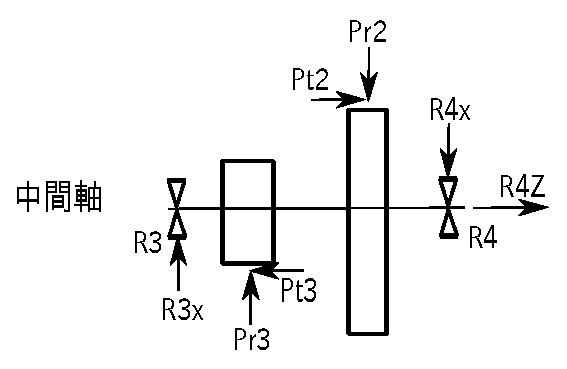
\includegraphics[width=10cm]{jiku43.eps}
\end{center}
\caption{中間軸モデル}
\end{figure}
釣り合いの式を以下に示す.
\begin{eqnarray}
x成分&:&P_{r3}-P_{r2}+R_{3x}-R_{4x}=0\\
y成分&:&-Fw_{12}-Fw_{34}+R_{3y}+R_{4y}=0\\
z成分&:&P_{t2}-P_{t3}+R_{4z}=0\\
y軸,R_3回りのモーメント&:&a_1P_{r3}-(a_1+a_2)P_{r2}+(a_1+a_2+a_3)R_{4x}+\frac{d_3}{2}P_{t3}+\frac{d_2}{2}P_{t2}\nonumber\\
\\
x軸,R_3回りのモーメント&:&a_1Fw_{34}+(a_1+a_2)Fw_{12}-(a_1+a_2+a_3)F_{4y}
\end{eqnarray}
この方程式を解くことで,次の結果を得る.
\begin{itemize}
\item $R_{3x} = 3529.680$
\item $R_{3y} = 6011.182$
\item $R_{4x} = 1520.624$
\item $R_{4y} = 4210.847$
\item $R_{4z} = 1978.130$
\end{itemize}
上の結果から,軸受けにかかるラジアル荷重の大きさが以下のように算出できる.
\begin{eqnarray}
R_3 &=& \sqrt {R_{3x}^2+R_{3y}^2}\\
    &=& \sqrt {3529.680^2+6011.182^2}=6970.865\\
R_4 &=& \sqrt {R_{4x}^2+R_{4y}^2}\\
    &=& \sqrt {1520.624^2+4210.847^2}=4477.000
\end{eqnarray}
次に,この軸にかかるモーメントを求め,BMDに示す.
歯車が有る点を中心に考えると,軸受けのラジアル力によって軸にかかるモーメントは次のように求めることができる.
\begin{figure}[htbp]
\begin{center}
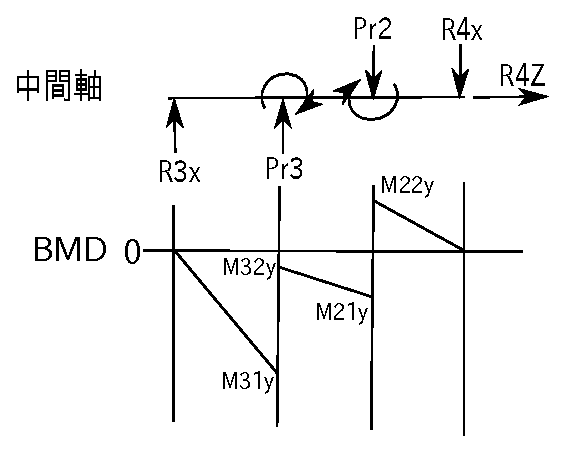
\includegraphics[width=10cm]{jiku44.eps}
\end{center}
\caption{中間軸y軸基準}
\end{figure}
\begin{figure}[htbp]
\begin{center}
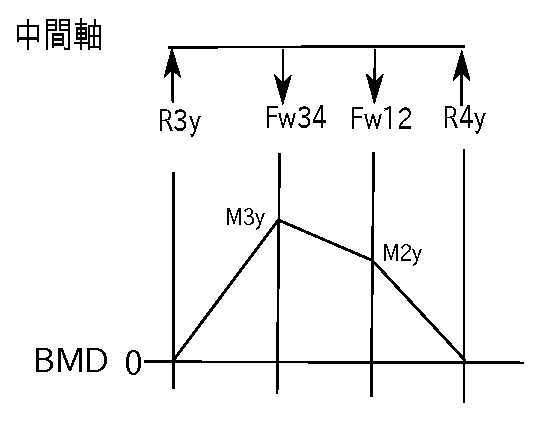
\includegraphics[width=10cm]{jiku46.eps}
\end{center}
\caption{中間軸x軸基準}
\end{figure}
\begin{eqnarray}
M_{3x} &=& R_{3y} \times a_1=405754.796\\
M_{4x} &=& R_{4y} \times (a_2+a_3)=280021.328\\
M_{31y} &=& R_{3x} \times a_1=-238253.403\\
M_{32y} &=& M_{31y} + P_t \frac{d_3}{2}=-48596.496\\
M_{21y} &=& M_{22y} + P_t \frac{d_2}{2}=88537.984\\
M_{22y} &=& R_{4x} \times a_3=101121.465
\end{eqnarray}
以上より,最大モーメントの組み合わせは,
\begin{eqnarray}
\sqrt{ M_{x3}^2 + M_{31y}^2 } = 470533.355
\end{eqnarray}
軸に作用するねじりモーメントを求める
\begin{eqnarray}
T_{3} &=& 0\\
T_{4} &=& \frac{d_3}{2} \times Fw_{34}\\
      &=& \frac{128.5374}{2} \times 7687.628 = 494073.883
\end{eqnarray}
軸に作用する荷重(軸力:スラスト力)を求める.
\begin{eqnarray}
T_{z3} &=& -1978.130\\
T_{z4} &=& R_{4z} = 1978.130
\end{eqnarray}

\subsection{出力軸}
\begin{figure}[htbp]
\begin{center}
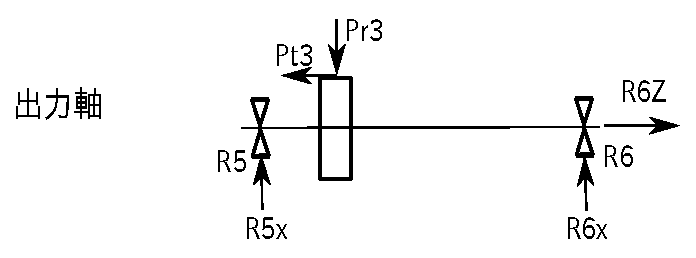
\includegraphics[width=10cm]{jiku3.eps}
\end{center}
\caption{出力軸モデル(xz成分)}
\end{figure}
\begin{figure}[htbp]
\begin{center}
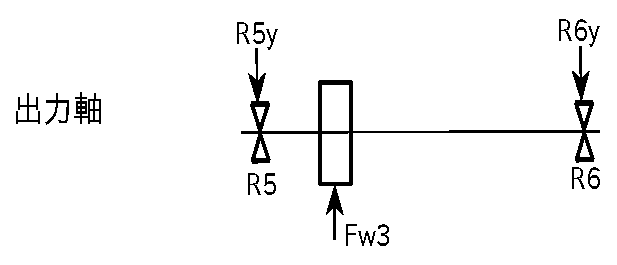
\includegraphics[width=10cm]{jiku32.eps}
\end{center}
\caption{出力軸モデル(y成分)}
\end{figure}
\subsubsection{正回転の場合}
釣り合いの式を以下に示す.
\begin{eqnarray}
x成分&:&-P_{r3}+R_{5x}+R_{6x}=0\\
y成分&:&Fw_{34}-R_{5y}-R_{6y}=0\\
z成分&:&-P_{t3}+R_{6z}=0\\
y軸,R_5回りのモーメント&:&-a_1P_{r3}+\frac{d_4}{2}P_{t3}+(a_1+a_2+a_3)R_{6x}\\
x軸,R_5回りのモーメント&:&a_1Fw_{34}-(a_1+a_2+a_3)R_{6y}
\end{eqnarray}
この方程式を解くことで,次の結果を得る.
\begin{itemize}
\item $R_{5x}=4789.314$
\item $R_{5y}=5204.782$
\item $R_{5z}=2951.000$
\item $R_{6x}=1792.187$
\item $R_{6y}=2482.846$
\end{itemize}
上の結果から,軸受けにかかるラジアル荷重の大きさが以下のように算出できる.
\begin{eqnarray}
R_5 &=& \sqrt {R_{5x}^2+R_{5y}^2}\\
    &=& \sqrt {4789.314^2+5204.782^2}=7072.996\\
R_6 &=& \sqrt {R_{6x}^2+R_{6y}^2}\\
    &=& \sqrt {-1792.187^2+2482.846^2}=3062.101
\end{eqnarray}
次に,この軸にかかるモーメントを求め,BMDに示す.
歯車が有る点を中心に考えると,軸受けのラジアル力によって軸にかかるモーメントは次のように求めることができる.
\begin{figure}[htbp]
\begin{center}
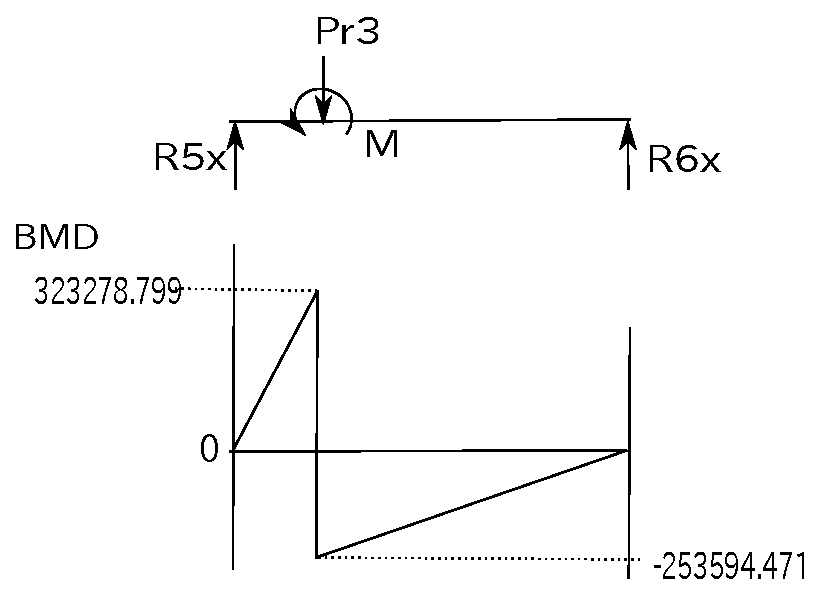
\includegraphics[width=12cm]{jiku34.eps}
\end{center}
\caption{入力軸モデル(x成分BMD)}
\end{figure}
\begin{figure}[htbp]
\begin{center}
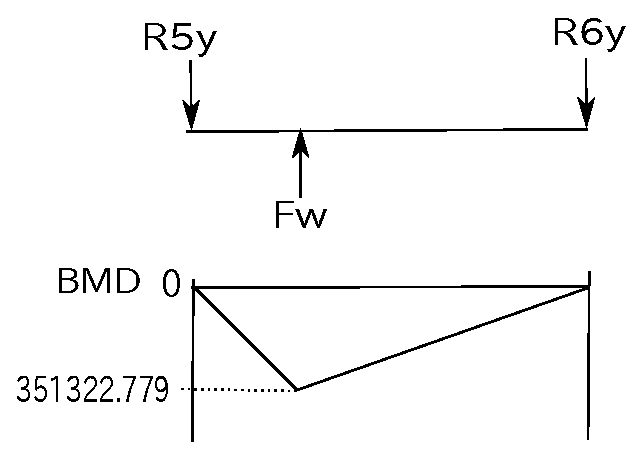
\includegraphics[width=9cm]{jiku33.eps}
\end{center}
\caption{入力軸モデル(y成分BMD)}
\end{figure}
\begin{eqnarray}
M_{5x} &=& R_{5y} \times a_1=351322.779\\
M_{6x} &=& R_{6y} \times (a_2+a_3)=351322.779\\
M_{5y} &=& R_{5x} \times a_1=323278.666\\
M_{6y} &=& R_{6x} \times (a_2+a_3)=-253594.471
\end{eqnarray}
最大曲げモーメントを算出する.
\begin{eqnarray}
M_{1max} &=& \sqrt {M_{5x}^2+M_{5y}^2}\\
         &=& \sqrt {351322.779^2+(323278.666)^2}=477427.262\\
M_{2max} &=& \sqrt {M_{6x}^2+M_{6y}^2}\\
         &=& \sqrt {351322.779^2+(-253594.471)^2}=433287.261
\end{eqnarray}
軸に作用するねじりモーメントを求める
\begin{eqnarray}
T_{1} &=& 0\\
T_{2} &=& \frac{d_4}{2} \times Fw_{34}\\
      &=& \frac{390.9679}{2} \times 7687.628 = 1502807.966
\end{eqnarray}
軸に作用する荷重(軸力:スラスト力)を求める.
\begin{eqnarray}
T_{z1} &=& 0\\
T_{z2} &=& R_{6z} = P_{t3} = 2951.000
\end{eqnarray}
\subsubsection{逆回転の場合}
釣り合いの式を以下に示す.
\begin{eqnarray}
x成分&:&-P_{r3}+R_{5x}+R_{6x}=0\\
y成分&:&Fw_{34}-R_{5y}-R_{6y}=0\\
z成分&:&-P_{t3}+R_{5z}=0\\
y軸,R_5回りのモーメント&:&-a_1P_{r3}+\frac{d_4}{2}P_{t3}+(a_1+a_2+a_3)R_{6x}\\
x軸,R_5回りのモーメント&:&a_1Fw_{34}-(a_1+a_2+a_3)R_{6y}
\end{eqnarray}
この方程式を解くことで,次の結果を得る.
\begin{itemize}
\item $R_{5x}=731.004$
\item $R_{5y}=-5204.782$
\item $R_{5z}=-2951.000$
\item $R_{6x}=-3728.130$
\item $R_{6y}=-2482.846$
\end{itemize}
上の結果から,軸受けにかかるラジアル荷重の大きさが以下のように算出できる.
\begin{eqnarray}
R_5 &=& \sqrt {R_{5x}^2+R_{5y}^2}\\
    &=& \sqrt {731.004^2+(-5204.782)^2}=5255.865\\
R_6 &=& \sqrt {R_{6x}^2+R_{6y}^2}\\
    &=& \sqrt {(-3728.130)^2+(-2482.846)^2}=4479.228
\end{eqnarray}
次に,この軸にかかるモーメントを求め,BMDに示す.
歯車が有る点を中心に考えると,軸受けのラジアル力によって軸にかかるモーメントは次のように求めることができる.
\begin{figure}[htbp]
\begin{center}
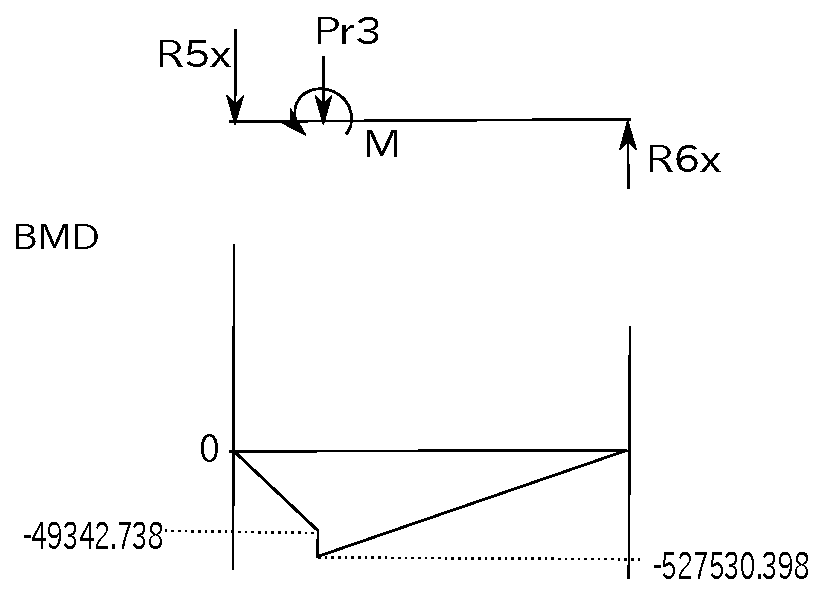
\includegraphics[width=12cm]{jiku342.eps}
\end{center}
\caption{入力軸モデル(x成分BMD)}
\end{figure}
\begin{figure}[htbp]
\begin{center}
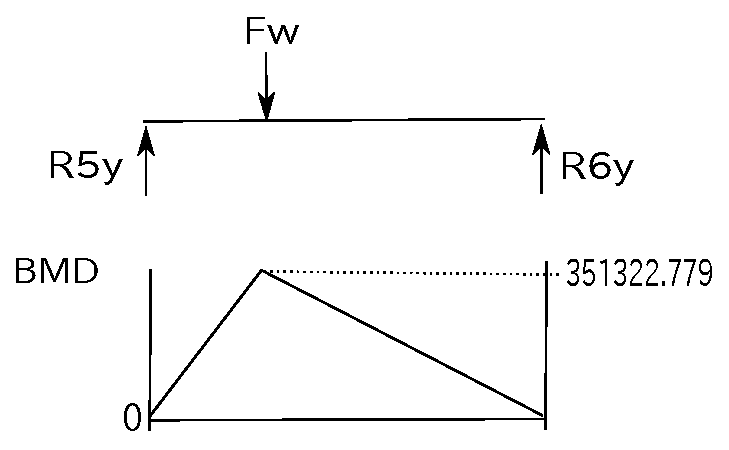
\includegraphics[width=9cm]{jiku332.eps}
\end{center}
\caption{入力軸モデル(y成分BMD)}
\end{figure}
\begin{eqnarray}
M_{5x} &=& R_{5y} \times a_1=351322.779\\
M_{6x} &=& R_{6y} \times (a_2+a_3)=351322.779\\
M_{5y} &=& R_{5x} \times a_1=49342.738\\
M_{6y} &=& R_{6x} \times (a_2+a_3)=-527530.398
\end{eqnarray}
最大曲げモーメントを算出する.
\begin{eqnarray}
M_{1max} &=& \sqrt {M_{5x}^2+M_{5y}^2}\\
         &=& \sqrt {351322.779^2+(49342.738)^2}=354770.913\\
M_{2max} &=& \sqrt {M_{6x}^2+M_{6y}^2}\\
         &=& \sqrt {351322.779^2+(-527530.398)^2}=633810.710
\end{eqnarray}
軸に作用するねじりモーメントを求める
\begin{eqnarray}
T_{1} &=& 0\\
T_{2} &=& \frac{d_4}{2} \times Fw_{34}\\
      &=& \frac{390.9679}{2} \times 7687.628 = 1502807.966
\end{eqnarray}
軸に作用する荷重(軸力:スラスト力)を求める.
\begin{eqnarray}
T_{z1} &=& 0\\
T_{z2} &=& R_{6z} = P_{t3} = 2951.000
\end{eqnarray}

\section{軸の最小径の決定}
\subsection{計算手順}
まず次の計算を行い,最小軸径をそれぞれ求める.
\begin{enumerate}
\item 破壊条件に基づく軸径\\
軸に生じる最大応力が,軸の許容応力よりも大きくなければならないという条件から,軸の最小径を求めていく.ここで用いる軸は丸棒であるので,軸の径が小さいほど許容せん断応力は小さくなる.よって,軸の直径dを小さくしていき,許容せん断応力と最大せん断応力が等しくなるdを算出すればよい.
\item 座屈条件に基づく軸径\\
座屈荷重による強度は,最小断面2次モーメントに依存する.これにより,耐えられる座屈荷重が決定するので,最小軸径も決定する.
\item ねじり剛性に基づく軸径\\
一般的に,1mの軸に対して0.25[degree]というのが目安になる.軸系を大きくするとねじられにくさが向上するので,最小軸系も決定する.
\end{enumerate}
それぞれ算出した軸径以上の軸径を選択する.また,入力軸の材料は第1歯車と一体化しなければならないので,第1歯車と同素材を用いる.よって軸の許容応力は以下のように定まる.キー溝が有る場合は,次の値に更に0.75倍したものを採用する.
\begin{eqnarray}
最大せん断応力の場合 \tau_{al} &=& 0.18 \times \sigma_{UTS}\\
&=&0.18 \times 755.1 = 135.92 [MPa]\\
最大主応力の場合 \tau_{al} &=& 0.36 \times \sigma_{UTS} \\
&=&0.36 \times 755.1 = 271.84[MPa]
\end{eqnarray}
\subsubsection{動的効果係数}
実際の軸にはどう荷重が作用する,この影響を考えるために,動的効果の係数を導入する.この係数は3段階に分類分けされているが,ここでは軽い変動荷重が作用するとして,ねじりの動的効果の係数を$k_t = 1.0,k_b = 1.5$として計算をする.
\subsection{破壊条件に基づく軸径}
軸受け1にかかる許容せん断応力$\tau_{al}$は,ねじりが作用しないので,次の式で算出する.
\begin{eqnarray}
\tau_{al} = \frac{16}{\pi d^3}\sqrt{(M+\frac{d}{8}P)^2+T^2}\\
軸径dについて解くと,\nonumber\\
d_{min} = \sqrt [3]{ \frac{16}{\pi \tau_{al}}\sqrt{(M+\frac{d}{8}P)^2+T^2} }\\
動的効果の係数に直すと,\nonumber\\
d_{min} = \sqrt [3]{ \frac{16}{\pi \tau_{al}}\sqrt{(k_bM+\frac{d}{8}P)^2+k_tT^2} }
\end{eqnarray}
\subsubsection{軸受け1側の軸(正回転)}
軸受け1側にかかる許容せん断応力$\tau_{al}$は,ねじりと軸力が作用しないので,次の式で算出する.ここで$P=0,T=0$を代入した.
\begin{eqnarray}
d_{11min} &=& \sqrt [3]{ \frac{16}{\pi \tau_{al}}\sqrt{k_bM^2} }\\
       &=& \sqrt [3]{ \frac{16}{\pi 135.92}\sqrt{1.5 \times 115549.168^2} }\\
       &=& 18.66[mm]
\end{eqnarray}
\subsubsection{軸受け1側の軸(逆回転)}
軸受け1側にかかる許容せん断応力$\tau_{al}$は,ねじりと軸力が作用しないので,次の式で算出する.ここで$P=0,T=0$を代入した.
\begin{eqnarray}
d_{11min} &=& \sqrt [3]{ \frac{16}{\pi \tau_{al}}\sqrt{k_bM^2} }\\
       &=& \sqrt [3]{ \frac{16}{\pi 135.92}\sqrt{1.5 \times 138595.08^2} }\\
       &=& 19.82[mm]
\end{eqnarray}
\subsubsection{軸受け2側の軸(正回転)}
軸受け2側にかかる許容せん断応力$\tau_{al}$は,ねじりと軸力が作用しないので,次の式で算出する.ここで$P=-972.87,T=124876.26, M=129657.71$を代入した.この計算ではd(直径)の値がわかっていないので,繰り返し計算で算出する.初期値20[mm]とする.
\begin{eqnarray}
d_{12min}&=& \sqrt [3]{ \frac{16}{\pi \tau_{al}}\sqrt{(k_bM+\frac{d}{8}P)^2+k_tT^2} }\\
       &=& \sqrt [3]{ \frac{16}{\pi 135.92} \sqrt{(1.5 \times 129657.71 +\frac{20}{8}\times -972.87)^2+(1.0 \times 124876.26)^2} }\\
       &=&20.47\\
       &=& \sqrt [3]{ \frac{16}{\pi 135.92} \sqrt{(1.5 \times 129657.71 +\frac{20.47}{8}\times -972.87)^2+(1.0 \times 124876.26)^2} }\\
       &=&20.47[mm](収束確認)
\end{eqnarray}
\subsubsection{軸受け2側の軸(逆回転)}
軸受け2側にかかる許容せん断応力$\tau_{al}$は,ねじりと軸力が作用しないので,次の式で算出する.ここで$P=972.87,T=124876.26, M=118650.16$を代入した.この計算ではd(直径)の値がわかっていないので,繰り返し計算で算出する.初期値20[mm]とする.
\begin{eqnarray}
d_{12min}&=& \sqrt [3]{ \frac{16}{\pi \tau_{al}}\sqrt{(k_bM+\frac{d}{8}P)^2+k_tT^2} }\\
       &=& \sqrt [3]{ \frac{16}{\pi 135.92} \sqrt{(1.5 \times 118650.16 +\frac{20}{8}\times 972.87)^2+(1.0 \times 124876.26)^2} }\\
       &=&20.18\\
       &=& \sqrt [3]{ \frac{16}{\pi 135.92} \sqrt{(1.5 \times 118650.16 +\frac{20.18}{8}\times 972.87)^2+(1.0 \times 124876.26)^2} }\nonumber\\
\\
       &=&20.18[mm](収束確認)
\end{eqnarray}
\subsubsection{軸受け3側の軸(正回転)}
軸受け33側にかかる許容せん断応力$\tau_{al}$は,ねじりと軸力が作用しないので,次の式で算出する.ここで$P=0,T=0$を代入した.
\begin{eqnarray}
d_{11min} &=& \sqrt [3]{ \frac{16}{\pi \tau_{al}}\sqrt{k_bM^2} }\\
         &=& \sqrt [3]{ \frac{16}{\pi 135.92}\sqrt{1.5 \times 405810.94^2} }\\
         &=& 28.36[mm]
\end{eqnarray}
\subsubsection{軸受け3側の軸(逆回転)}
軸受け3側にかかる許容せん断応力$\tau_{al}$は,ねじりと軸力が作用しないので,次の式で算出する.ここで$P=0,T=0$を代入した.
\begin{eqnarray}
d_{11min} &=& \sqrt [3]{ \frac{16}{\pi \tau_{al}}\sqrt{k_bM^2} }\\
         &=& \sqrt [3]{ \frac{16}{\pi 135.92}\sqrt{1.5 \times 470533.23^2} }\\
         &=& 29.79[mm]
\end{eqnarray}
\subsubsection{第3歯車と第4歯車の間の軸(正回転)}
軸受け3側にかかる許容せん断応力$\tau_{al}$は,ねじりと軸力が作用しないので,次の式で算出する.また,キー溝があるので,$\tau_{al}$の値を0.75倍にした.ここで$P=2951,T=494077.63, M=445071.18$を代入した.この計算ではd(直径)の値がわかっていないので,繰り返し計算で算出する.初期値20[mm]とする.
\begin{eqnarray}
d_{12min}&=& \sqrt [3]{ \frac{16}{\pi \tau_{al}}\sqrt{(k_bM+\frac{d}{8}P)^2+k_tT^2} }\\
       &=& \sqrt [3]{ \frac{16}{\pi \times 0.75 \times 135.92} \sqrt{(1.5 \times 445071.18 +\frac{20}{8}\times -2951)^2+(1.0 \times 494077.63)^2} }\nonumber\\
\\
       &=&34.53\\
       &=& \sqrt [3]{ \frac{16}{\pi \times 0.75 \times 135.92} \sqrt{(1.5 \times 445071.18 +\frac{34.53}{8}\times -2951)^2+(1.0 \times 494077.63)^2} }\nonumber\\
\\
         &=& 34.48[mm]\\
       &=& \sqrt [3]{ \frac{16}{\pi \times 0.75 \times 135.92} \sqrt{(1.5 \times 445071.18 +\frac{34.48}{8}\times -2951)^2+(1.0 \times 494077.63)^2} }\nonumber\\
\\
         &=& 34.48[mm](収束確認)
\end{eqnarray}
\subsubsection{第3歯車と第4歯車の間の軸(逆回転)}
軸受け3側にかかる許容せん断応力$\tau_{al}$は,ねじりと軸力が作用しないので,次の式で算出する.また,キー溝があるので,$\tau_{al}$の値を0.75倍にした.ここで$P=2951,T=, M=408654.51$を代入した.この計算ではd(直径)の値がわかっていないので,繰り返し計算で算出する.初期値20[mm]とする.
\begin{eqnarray}
d_{12min}&=& \sqrt [3]{ \frac{16}{\pi \tau_{al}}\sqrt{(k_bM+\frac{d}{8}P)^2+k_tT^2} }\\
       &=& \sqrt [3]{ \frac{16}{\pi \times 0.75 \times 135.92} \sqrt{(1.5 \times 408654.51 +\frac{20}{8}\times 2951)^2+(1.0 \times 494077.63)^2} }\nonumber\\
\\
       &=&34.09\\
       &=& \sqrt [3]{ \frac{16}{\pi \times 0.75 \times 135.92} \sqrt{(1.5 \times 408654.51 +\frac{34.09}{8}\times 2951)^2+(1.0 \times 494077.63)^2} }\nonumber\\
\\
         &=& 34.10[mm](収束確認)
\end{eqnarray}
\subsubsection{第4歯車側の軸(正回転)}
軸受け4側にかかる許容せん断応力$\tau_{al}$は,ねじりと軸力が作用しないので,次の式で算出する.また,キー溝があるので,$\tau_{al}$の値を0.75倍にした.ここで$P=-1978.13,M=313185.59$を代入した.この計算ではd(直径)の値がわかっていないので,繰り返し計算で算出する.初期値20[mm]とする.
\begin{eqnarray}
d_{12min}&=& \sqrt [3]{ \frac{16}{\pi \tau_{al}}\sqrt{(k_bM+\frac{d}{8}P)^2+k_tT^2} }\\
       &=& \sqrt [3]{ \frac{16}{\pi \times 135.92} \sqrt{(1.5 \times 313185.59 +\frac{20}{8}\times -1978.13)^2}}\nonumber\\
\\
       &=&25.92\\
       &=& \sqrt [3]{ \frac{16}{\pi \times 135.92} \sqrt{(1.5 \times 313185.59 +\frac{25.92}{8}\times -1978.13)^2} }\nonumber\\
\\
         &=& 25.89[mm]\\
       &=& \sqrt [3]{ \frac{16}{\pi \times 135.92} \sqrt{(1.5 \times 313185.59 +\frac{34.48}{8}\times -1978.13)^2} }\nonumber\\
\\
         &=& 25.89[mm](収束確認)
\end{eqnarray}
\subsubsection{第4歯車側の軸(逆回転)}
軸受け4側にかかる許容せん断応力$\tau_{al}$は,ねじりと軸力が作用しないので,次の式で算出する.また,キー溝があるので,$\tau_{al}$の値を0.75倍にした.ここで$P=1978.13,M=297720.25$を代入した.この計算ではd(直径)の値がわかっていないので,繰り返し計算で算出する.初期値20[mm]とする.
\begin{eqnarray}
d_{12min}&=& \sqrt [3]{ \frac{16}{\pi \tau_{al}}\sqrt{(k_bM+\frac{d}{8}P)^2} }\\
       &=& \sqrt [3]{ \frac{16}{\pi \times 135.92} \sqrt{(1.5 \times 297720.25 +\frac{20}{8}\times 1978.13)^2}}\nonumber\\
\\
       &=& 25.67\\
       &=& \sqrt [3]{ \frac{16}{\pi  \times 135.92} \sqrt{(1.5 \times 297720.25 +\frac{34.09}{8}\times 1978.13)^2}}\nonumber\\
\\
         &=& 25.67[mm](収束確認)
\end{eqnarray}
\subsubsection{第5歯車側の軸(正回転)}
軸受け3側にかかる許容せん断応力$\tau_{al}$は,ねじりと軸力が作用しないので,次の式で算出する.また,キー溝があるので,$\tau_{al}$の値を0.75倍にした.ここで$P=2951,T=1502808.35, M=477427.46$を代入した.この計算ではd(直径)の値がわかっていないので,繰り返し計算で算出する.初期値20[mm]とする.
\begin{eqnarray}
d_{12min}&=& \sqrt [3]{ \frac{16}{\pi \tau_{al}}\sqrt{(k_bM+\frac{d}{8}P)^2+k_tT^2} }\\
       &=& \sqrt [3]{ \frac{16}{\pi \times 0.75 \times 135.92} \sqrt{(1.5 \times 477427.46 +\frac{20}{8}\times 2951)^2+(1.0 \times 1502808.35)^2} }\nonumber\\
\\
       &=&43.71\\
       &=& \sqrt [3]{ \frac{16}{\pi \times 0.75 \times 135.92} \sqrt{(1.5 \times 477427.46 +\frac{42.41}{8}\times 2951)^2+(1.0 \times 1502808.35)^2} }\nonumber\\
\\
       &=& 43.71[mm](収束確認)\\
\end{eqnarray}
\subsubsection{第5歯車側の軸(正回転)}
軸受け3側にかかる許容せん断応力$\tau_{al}$は,ねじりと軸力が作用しないので,次の式で算出する.また,キー溝があるので,$\tau_{al}$の値を0.75倍にした.ここで$P=-2951,T=1502808.35,M=354770.75$を代入した.この計算ではd(直径)の値がわかっていないので,繰り返し計算で算出する.初期値20[mm]とする.
\begin{eqnarray}
d_{12min}&=& \sqrt [3]{ \frac{16}{\pi \tau_{al}}\sqrt{(k_bM+\frac{d}{8}P)^2+k_tT^2} }\\
       &=& \sqrt [3]{ \frac{16}{\pi \times 0.75 \times 135.92} \sqrt{(1.5 \times 354770.75 +\frac{20}{8}\times -2951)^2+(1.0 \times 1502808.35)^2} }\nonumber\\
\\
       &=& 43.01\\
       &=& \sqrt [3]{ \frac{16}{\pi \times 0.75 \times 135.92} \sqrt{(1.5 \times 354770.75 +\frac{34.09}{8}\times -2951)^2+(1.0 \times 1502808.35)^2} }\nonumber\\
\\
         &=& 42.98[mm](収束確認)
\end{eqnarray}

\subsubsection{軸受け6側の軸(正回転)}
軸受け6側にかかる許容せん断応力$\tau_{al}$は,ねじりと軸力が作用しないので,次の式で算出する.ここで$P=0,T=0$を代入した.
\begin{eqnarray}
d_{11min} &=& \sqrt [3]{ \frac{16}{\pi \tau_{al}}\sqrt{k_bM^2} }\\
       &=& \sqrt [3]{ \frac{16}{\pi 135.92}\sqrt{1.5 \times 433286.99^2} }\\
       &=& 28.99[mm]
\end{eqnarray}
\subsubsection{軸受け6側の軸(逆回転)}
軸受け6側にかかる許容せん断応力$\tau_{al}$は,ねじりと軸力が作用しないので,次の式で算出する.ここで$P=0,T=0$を代入した.
\begin{eqnarray}
d_{11min} &=& \sqrt [3]{ \frac{16}{\pi \tau_{al}}\sqrt{k_bM^2} }\\
       &=& \sqrt [3]{ \frac{16}{\pi 135.92}\sqrt{1.5 \times 633810.96^2} }\\
       &=& 32.90[mm]
\end{eqnarray}

\subsection{座屈条件に基づく軸径}
\subsubsection{原理}
炭素鋼には,軟鋼と硬鋼があり,それぞれさらに特別極軟鋼,極軟鋼,軟鋼,半軟鋼,半硬鋼,硬鋼,最硬鋼と分類される.今回軸として採用した軸の材料はs53c(炭素量が0.53\%)であるので,最硬鋼に分類される.硬鋼の場合は,細長比が$85 \sqrt n$よりも小さければ,座屈で計算する.nは端末係数である.\\
\par
ここで,細長比$\lambda$は次のように算出する.
\begin{eqnarray}
\lambda &=& \frac{L}{r}\\
&&ここに,L:部材の長さ,r:断面回転半径\\
r&=&\sqrt{\frac{I}{A}}\\
&&ここに,A:断面積,I:断面2次モーメントとする.以上より,\\
\lambda &=& \frac{L\sqrt{A}}{\sqrt{I}}
\end{eqnarray}
座屈で計算する場合は,以下のオイラーの座屈公式を用いる.
\begin{eqnarray}
P_k &=& C\frac{\pi^2}{l^2}EI\\
I&=&\frac{\pi d^4}{64}\\
d&=&\sqrt[4]{P_k\frac{64l[mm^2]}{\pi^3CE[N/mm^2]}}
\end{eqnarray}
\subsubsection{第2軸受け側の軸}
\begin{eqnarray}
d&=&\sqrt[4]{P_k\frac{64l[mm^2]}{\pi^3CE[N/mm^2]}}\\
 &=&\sqrt[4]{972.87 \times \frac{64\times 66.5^2}{\pi^3 \times 206000[N/mm^2]}}\\
 &=&2.56[mm]
\end{eqnarray}
\subsubsection{第3軸受けと第4軸受けの間の軸}
\begin{eqnarray}
d&=&\sqrt[4]{P_k\frac{64l[mm^2]}{\pi^3CE[N/mm^2]}}\\
 &=&\sqrt[4]{2951 \times \frac{64\times 75^2}{\pi^3 \times 206000[N/mm^2]}}\\
 &=&3.59[mm]
\end{eqnarray}
\subsubsection{第4軸受け側の軸}
\begin{eqnarray}
d&=&\sqrt[4]{P_k\frac{64l[mm^2]}{\pi^3CE[N/mm^2]}}\\
 &=&\sqrt[4]{1978.13 \times \frac{64\times 66.5^2}{\pi^3 \times 206000[N/mm^2]}}\\
 &=&3.06[mm]
\end{eqnarray}
\subsubsection{第5軸受け側の軸}
\begin{eqnarray}
d&=&\sqrt[4]{P_k\frac{64l[mm^2]}{\pi^3CE[N/mm^2]}}\\
 &=&\sqrt[4]{2951 \times \frac{64\times 67.5^2}{\pi^3 \times 206000[N/mm^2]}}\\
 &=&3.41[mm]
\end{eqnarray}
\subsection{ねじり剛性に基づく軸径}
\subsubsection{計算原理}
上で述べたとおり,一般的な比ねじれ角の目安である$\bar{\theta} = 0.25\pi /180 [radian/m]$を採用して,次の計算をする.
\begin{eqnarray}
\bar{\theta} &=& \frac{T}{GJ}\\
&&ここで,J:断面2次極モーメント,G:縦弾性係数\\
J&=&\frac{\pi d^4}{32}\\
d[mm]&=&\sqrt[4]{\frac{32T[N \cdot mm]}{\pi \bar{\theta}/1000[radian/mm] G[N/mm^2]}}
\end{eqnarray}
以下の計算では,$G=79500[N/mm^2]$を用いて計算をする.
\subsubsection{軸受け2側の軸}
\begin{eqnarray}
d[mm]&=&\sqrt[4]{\frac{32T[N \cdot mm]}{\pi \bar{\theta}/1000[radian/mm] G[N/mm^2]}}\\
     &=&\sqrt[4]{\frac{32\times 124876.26 }{\pi \times 0.25/1000 \times 79500}}\\
     &=&43.76[mm]
\end{eqnarray}
\subsubsection{第2歯車と第3歯車の間の軸}
\begin{eqnarray}
d[mm]&=&\sqrt[4]{\frac{32T[N \cdot mm]}{\pi \bar{\theta}/1000[radian/mm] G[N/mm^2]}}\\
     &=&\sqrt[4]{\frac{32\times 494077.63 }{\pi \times 0.25/1000 \times 79500}}\\
     &=&61.72[mm]
\end{eqnarray}
\subsubsection{軸受け5側の軸}
\begin{eqnarray}
d[mm]&=&\sqrt[4]{\frac{32T[N \cdot mm]}{\pi \bar{\theta}/1000[radian/mm] G[N/mm^2]}}\\
     &=&\sqrt[4]{\frac{32\times 1502808.35 }{\pi \times 0.25/1000 \times 79500}}\\
     &=&81.5[mm]
\end{eqnarray}
\section{最小軸径のまとめ}
\begin{table}[htb]
\begin{center}
  \caption{最小軸径のまとめ}
  \begin{tabular}{|l||c|c|} \hline
軸の名称&軸の最小径[mm]&軸の径[mm]\\\hline\hline
d11&19.82&20\\
d12&43.76&44\\
d21&29.79&30\\
d22&61.72&62\\
d23&25.89&26\\
d31&81.5&82\\
d32&32.9&33\\
\hline
  \end{tabular}
\end{center}
\end{table}
\section{キーの設計}
\subsection{キーの許容圧縮応力と許容せん断応力}
キーに使う材料は,s45c(機械構造用炭素鋼鋼材)とし,端部は角型とする.安産率は4とする.キーの許容圧縮応力と許容せん断応力の計算を以下に示す.
\begin{eqnarray}
(s45cの引っ張り強さ)&=&690[N/mm^2]\\
キーの許容圧縮応力:\sigma_{al} = \frac{690}{4} &=& 172.5[N/mm^2]\\
許容せん断応力:\tau_{al}=\frac{\sigma_{al}}{2} &=& 86.25[N/mm^2]
\end{eqnarray}
次の関係式を満たすようにキーを設計する。
\begin{eqnarray}
\sigma_{al} \geq \frac{2T}{dlt_1}\\
\nonumber\\
\tau_{al} \geq \frac{2T}{dlb}
\end{eqnarray}
\subsection{第2歯車のキー}
d=62,b=18,h=11,l=50と仮定すると、
\begin{eqnarray}
\sigma_{al} &\geq& \frac{2T}{dlt_1}\\
(右辺) &=& \frac{2 \times 494077.63[N \cdot mm]}{62[mm] \times 50[mm] \times 11/2[mm]}\\
       &\approx&57.956[N \cdot m]\\
       &\leq& 172.5\\
\tau_{al} &\geq& \frac{2T}{dlb}\\
(右辺) &=& \frac{2 \times 494077.63[N \cdot mm]}{62[mm] \times 50[mm] \times 18[mm]}\\
       &=& 17.70\\
       &\leq&86.25[N \cdot m]
\end{eqnarray}
よって、仮定値を採用する
\subsection{第3歯車のキー}
d=62,b=18,h=11,l=50と仮定すると、
\begin{eqnarray}
\sigma_{al} &\geq& \frac{2T}{dlt_1}\\
(右辺) &=& \frac{2 \times 494077.63[N \cdot mm]}{62[mm] \times 50[mm] \times 11/2[mm]}\\
       &\approx&57.956[N \cdot m]\\
       &\leq& 172.5\\
\tau_{al} &\geq& \frac{2T}{dlb}\\
(右辺) &=& \frac{2 \times 494077.63[N \cdot mm]}{62[mm] \times 50[mm] \times 18[mm]}\\
       &=& 17.70\\
       &\leq&86.25[N \cdot m]
\end{eqnarray}
よって、仮定値を採用する
\subsection{第4歯車のキー}
d=82,b=22,h=14,l=70と仮定すると、
\begin{eqnarray}
\sigma_{al} &\geq& \frac{2T}{dlt_1}\\
(右辺) &=& \frac{2 \times 1502808.35015[N \cdot mm]}{82[mm] \times 70[mm] \times 14/2[mm]}\\
       &\approx&74.804[N \cdot m]\\
       &\leq& 172.5\\
\tau_{al} &\geq& \frac{2T}{dlb}\\
(右辺) &=& \frac{2 \times 1502808.35015[N \cdot mm]}{82[mm] \times 70[mm] \times 22[mm]}\\
       &=& 23.801\\
       &\leq&86.25[N \cdot m]
\end{eqnarray}
よって、仮定値を採用する

\chapter{軸受け}
\section{軸受けにかかる力のまとめ}
\begin{table}[htb]
\begin{center}
  \caption{表題}
  \begin{tabular}{|l||c|c|c|c|} \hline
軸受け番号& 最小軸径[mm] &ラジアル荷重Fr[N] &スラスト荷重Fa[N]&回転数[rpm]\\\hline
1&20&972.6&0&1300\\
2&44&1784.21&972.87&1300\\
3&30&6970.86&0&328.5714\\
4&26&4477&1978.13&328.5714\\
5&82&5255.86&2951&108.0235\\
6&33&4479.24&0&108.0235\\
\hline
  \end{tabular}
\end{center}
\end{table}

\section{軸受け計算}
\newpage
\subsection{軸受け1の選定}
\subsubsection{軸受け1データ}
\begin{table}[htb]
\begin{center}
  \caption{軸受け1データ}
  \begin{tabular}{lll} \hline
名称&記号&値\\
ラジアル荷重&$F_r$&972.6[N]\\
スラスト荷重&$F_a$&0\\
回転数&n&1300[rpm]\\
定格寿命&$L_h$&20000以上 [hour]\\
最小軸径&$\alpha$&20 [mm]\\
軸受け種類&p(玉軸受け)&3[$\cdot$]\\
\hline
  \end{tabular}
\end{center}
\end{table}

\begin{table}[htb]
\begin{center}
  \caption{NSK60/28}
  \begin{tabular}{lll} \hline
名称&記号&値\\
内径& d &28 [mm]\\
外径& D &52 [mm]\\
基本動定格荷重&$C_{r}$&12500\\
基本静定格荷重&$C_{0r}$&7400\\
軸受各部の形状および適用する&$f_0$&14.5\\
応力水準によって定まる係数&&\\
\hline
  \end{tabular}
\end{center}
\end{table}


\subsubsection{軸受け1検討}
\begin{eqnarray}
寿命係数f_h &=& \left( \frac{L_h}{500} \right)^{1/p} = \left( \frac{20000}{500} \right)^{1/3} = 3.420\\
速度係数f_n &=& \left( \frac{100}{3n} \right)^{1/p} = \left( \frac{100}{3 \times 1300} \right)^{1/3} = 0.29488\\
P &=& XF_r+YF_a = 972.6\\
C &=& \frac{f_h}{f_n} \times P = 11280.1546[N]
\end{eqnarray}

\subsubsection{軸受け1再検討}
アキシアル荷重が働いていないので、自動的にX=1,Y=0とする。
\begin{eqnarray}
寿命時間L_h &=& 500{f_n}^p(C_r/P)^p\\
           &=& 500 \times \frac{100}{3 \times 1300} \times (12500/972.6)^3\\
           &=& 27126.523 \geq 20000
\end{eqnarray}

\subsubsection{静荷重の確認}
\begin{eqnarray}
0.6F_r+0.5F_a=0.6 \times 972.6 + 0.5 \times 0 = 486.3 \leq F_r\\
よって、静等価荷重P_0 = F_r=972.6\\
f_s = \frac{C_{0r}}{P_0} = \frac{7400}{972.6}\geq 1
\end{eqnarray}

\newpage
\subsection{軸受け2の選定}
\subsubsection{軸受け2データ}
\begin{table}[htb]
\begin{center}
  \caption{軸受け2データ}
  \begin{tabular}{lll} \hline
名称&記号&値\\
ラジアル荷重&$F_r$&1784.21[N]\\
スラスト荷重&$F_a$&972.87[N]\\
回転数&n&328.5714[rpm]\\
定格寿命&$L_h$&20000以上 [hour]\\
最小軸径&$\alpha$&44 [mm]\\
軸受け種類&p(玉軸受け)&3[$\cdot$]\\
\hline
  \end{tabular}
\end{center}
\end{table}

\begin{table}[htb]
\begin{center}
  \caption{NSK6011}
  \begin{tabular}{lll} \hline
名称&記号&値\\
内径& d &55 [mm]\\
外径& D &90 [mm]\\
基本動定格荷重&$C_{r}$&28300\\
基本静定格荷重&$C_{0r}$&21200\\
軸受各部の形状および適用する&$f_0$&15.3\\
応力水準によって定まる係数&&\\
\hline
  \end{tabular}
\end{center}
\end{table}


\subsubsection{軸受け2検討}
X=0.56,Y=1.00とする。
\begin{eqnarray}
寿命係数f_h &=& \left( \frac{L_h}{500} \right)^{1/p} = \left( \frac{20000}{500} \right)^{1/3} = 3.420\\
速度係数f_n &=& \left( \frac{100}{3n} \right)^{1/p} = \left( \frac{100}{3 \times 1300} \right)^{1/3} = 0.29488\\
\frac{F_a}{F_r} &=& \frac{972.87}{1784.21} = 0.5453(\geq 0.44)\\
P &=& XF_r+YF_a = 0.56 \times 1784.21 + 1.00 \times 972.87 = 1972.0276\\
C &=& \frac{f_h}{f_n} \times P = 11.59794 \times 1972.0276 = 22941.045[N]
\end{eqnarray}

\subsubsection{軸受け2再検討}
\begin{eqnarray}
寿命時間L_h &=& 500{f_n}^p(C_r/P)^p\\
           &=& 500 \times \frac{100}{3 \times 1300} \times (28300/1972.0276)^3\\
           &=& 37890.099 \geq 20000
\end{eqnarray}

\subsubsection{静荷重の確認}
\begin{eqnarray}
P_0&=&0.6F_r+0.5F_a\\
&=&0.6 \times 1784.21 + 0.5 \times 972.87 = 1556.961 \leq F_r\\
よって、静等価荷重P_0 &=& F_r =1784.21\\
f_s &=& \frac{C_{0r}}{P_0} = \frac{21200}{1784.21}\geq 1
\end{eqnarray}











\newpage
\subsection{軸受け3の選定}

\subsubsection{軸受け3データ}
\begin{table}[htb]
\begin{center}
  \caption{軸受け3データ}
  \begin{tabular}{lll} \hline
名称&記号&値\\
ラジアル荷重&$F_r$&6970.86[N]\\
スラスト荷重&$F_a$&0\\
回転数&n&328.5714[rpm]\\
定格寿命&$L_h$&20000以上 [hour]\\
最小軸径&$\alpha$&30 [mm]\\
軸受け種類&p(玉軸受け)&3[$\cdot$]\\
\hline
  \end{tabular}
\end{center}
\end{table}

\begin{table}[htb]
\begin{center}
  \caption{NSK6309}
  \begin{tabular}{lll} \hline
名称&記号&値\\
内径& d &45 [mm]\\
外径& D &100 [mm]\\
基本動定格荷重&$C_{r}$&53000\\
基本静定格荷重&$C_{0r}$&32000\\
軸受各部の形状および適用する&$f_0$&13.1\\
応力水準によって定まる係数&&\\
\hline
  \end{tabular}
\end{center}
\end{table}

\subsubsection{軸受け3検討}
\begin{eqnarray}
寿命係数f_h &=& \left( \frac{L_h}{500} \right)^{1/p} = \left( \frac{20000}{500} \right)^{1/3} = 3.420\\
速度係数f_n &=& \left( \frac{100}{3n} \right)^{1/p} = \left( \frac{100}{3 \times 328.5714} \right)^{1/3} = 0.4664\\
P &=& XF_r+YF_a = 6970.86\\
C &=& \frac{f_h}{f_n} \times P = 51115.654[N]
\end{eqnarray}

\subsubsection{軸受け3再検討}
アキシアル荷重が働いていないので、自動的にX=1,Y=0とする。
\begin{eqnarray}
寿命時間L_h &=& 500{f_n}^p(C_r/P)^p\\
           &=& 500 \times \frac{100}{3 \times 328.5714} \times (53000/6970.86)^3\\
           &=& 22293.975 \geq 20000
\end{eqnarray}

\subsubsection{静荷重の確認}
\begin{eqnarray}
0.6F_r+0.5F_a=0.6 \times 6970.86 + 0.5 \times 0 = 4182.516 \leq F_r\\
よって、静等価荷重P_0 = F_r = 6970.86\\
f_s = \frac{C_{0r}}{P_0} = \frac{32000}{6970.86} \geq 1
\end{eqnarray}

\newpage
\subsection{軸受け4の選定}
\subsubsection{軸受け4データ}
\begin{table}[htb]
\begin{center}
  \caption{軸受け4データ}
  \begin{tabular}{lll} \hline
名称&記号&値\\
ラジアル荷重&$F_r$&4477[N]\\
スラスト荷重&$F_a$&1978.13[N]\\
回転数&n&328.5714[rpm]\\
定格寿命&$L_h$&20000以上 [hour]\\
最小軸径&$\alpha$&26 [mm]\\
軸受け種類&p(玉軸受け)&3[$\cdot$]\\
\hline
  \end{tabular}
\end{center}
\end{table}

\begin{table}[htb]
\begin{center}
  \caption{NSK6308}
  \begin{tabular}{lll} \hline
名称&記号&値\\
内径& d &40 [mm]\\
外径& D &90 [mm]\\
基本動定格荷重&$C_{r}$&40500\\
基本静定格荷重&$C_{0r}$&24000\\
軸受各部の形状および適用する&$f_0$&13.2\\
応力水準によって定まる係数&&\\
\hline
  \end{tabular}
\end{center}
\end{table}

\subsubsection{軸受け4検討}
X=0.56,Y=1.00とする。
\begin{eqnarray}
寿命係数f_h &=& \left( \frac{L_h}{500} \right)^{1/p} = \left( \frac{20000}{500} \right)^{1/3} = 3.420\\
速度係数f_n &=& \left( \frac{100}{3n} \right)^{1/p} = \left( \frac{100}{3 \times 328.5714} \right)^{1/3} = 0.4664\\
\frac{F_a}{F_r} &=& \frac{1978.13}{4477} = 0.4418(\geq 0.44)\\
P &=& XF_r+YF_a = 0.56 \times 4477 + 1.00 \times 1978.13 = 4485.25\\
C &=& \frac{f_h}{f_n} \times P = 7.33276 \times 4485.25 = 32889.26[N]
\end{eqnarray}

\subsubsection{軸受け4再検討}
\begin{eqnarray}
寿命時間L_h &=& 500{f_n}^p(C_r/P)^p\\
           &=& 500 \times \frac{100}{3 \times 328.5714} \times (40500/4485.25)^3\\
           &=& 37344.2805 \geq 20000
\end{eqnarray}

\subsubsection{静荷重の確認}
\begin{eqnarray}
P_0&=&0.6F_r+0.5F_a\\
&=&0.6 \times 4477 + 0.5 \times 1978.13 = 3675.265 \leq F_r\\
よって、静等価荷重P_0 &=& F_r = 4477\\
f_s &=& \frac{C_{0r}}{P_0} = \frac{24000}{4477}\geq 1
\end{eqnarray}


\newpage
\subsection{軸受け5の選定}
\subsubsection{軸受け5データ}
\begin{table}[htb]
\begin{center}
  \caption{軸受け5データ}
  \begin{tabular}{lll} \hline
名称&記号&値\\
ラジアル荷重&$F_r$&5255.86[N]\\
スラスト荷重&$F_a$&2951[N]\\
回転数&n&108.0235[rpm]\\
定格寿命&$L_h$&20000以上 [hour]\\
最小軸径&$\alpha$&82 [mm]\\
軸受け種類&p(玉軸受け)&3[$\cdot$]\\
\hline
  \end{tabular}
\end{center}
\end{table}

\begin{table}[htb]
\begin{center}
  \caption{NSK6918}
  \begin{tabular}{lll} \hline
名称&記号&値\\
内径& d & 90 [mm]\\
外径& D & 125 [mm]\\
基本動定格荷重&$C_{r}$&3300\\
基本静定格荷重&$C_{0r}$&31500\\
軸受各部の形状および適用する&$f_0$&136.5\\
応力水準によって定まる係数&&\\
\hline
  \end{tabular}
\end{center}
\end{table}

\subsubsection{軸受け5検討}
X=0.56,Y=1.00とする。
\begin{eqnarray}
寿命係数f_h &=& \left( \frac{L_h}{500} \right)^{1/p} = \left( \frac{20000}{500} \right)^{1/3} = 3.420\\
速度係数f_n &=& \left( \frac{100}{3n} \right)^{1/p} = \left( \frac{100}{3 \times 108.0235} \right)^{1/3} = 0.67575\\
\frac{F_a}{F_r} &=& \frac{2986}{5255.86} = 0.568(\geq 0.44)\\
P &=& XF_r+YF_a = 0.56 \times 5255.86 + 1.00 \times 2951 = 5894.2816\\
C &=& \frac{f_h}{f_n} \times P = 5.0610 \times 5894.2816 = 29830.959[N]
\end{eqnarray}

\subsubsection{軸受け5再検討}
\begin{eqnarray}
寿命時間L_h &=& 500{f_n}^p(C_r/P)^p\\
           &=& 500 \times \frac{100}{3 \times 108.0235} \times (33000/5894.2816)^3\\
           &=& 27575.70 \geq 20000
\end{eqnarray}

\subsubsection{静荷重の確認}
\begin{eqnarray}
P_0&=&0.6F_r+0.5F_a\\
&=&0.6 \times 5255.86 + 0.5 \times 2951 = 4629.016 \leq F_r\\
よって、静等価荷重P_0 &=& F_r = 5255.86\\
f_s &=& \frac{C_{0r}}{P_0} = \frac{31500}{5255.86}\geq 1
\end{eqnarray}


\newpage
\subsection{軸受け6の選定}

\subsubsection{軸受け6データ}
\begin{table}[htb]
\begin{center}
  \caption{軸受け6データ}
  \begin{tabular}{lll} \hline
名称&記号&値\\
ラジアル荷重&$F_r$&4479.24[N]\\
スラスト荷重&$F_a$&0\\
回転数&n&108.0235[rpm]\\
定格寿命&$L_h$&20000以上 [hour]\\
最小軸径&$\alpha$&33 [mm]\\
軸受け種類&p(玉軸受け)&3[$\cdot$]\\
\hline
  \end{tabular}
\end{center}
\end{table}

\begin{table}[htb]
\begin{center}
  \caption{NSK6310}
  \begin{tabular}{lll} \hline
名称&記号&値\\
内径& d &50 [mm]\\
外径& D &110 [mm]\\
基本動定格荷重&$C_{r}$&62000\\
基本静定格荷重&$C_{0r}$&38500\\
軸受各部の形状および適用する&$f_0$&13.2\\
応力水準によって定まる係数&&\\
\hline
  \end{tabular}
\end{center}
\end{table}


\subsubsection{軸受け6検討}
\begin{eqnarray}
寿命係数f_h &=& \left( \frac{L_h}{500} \right)^{1/p} = \left( \frac{20000}{500} \right)^{1/3} = 3.420\\
速度係数f_n &=& \left( \frac{100}{3n} \right)^{1/p} = \left( \frac{100}{3 \times 108.0235} \right)^{1/3} = 0.67575\\
P &=& XF_r+YF_a = 4479.24\\
C &=& \frac{f_h}{f_n} \times P = 22669.62752[N]
\end{eqnarray}

\subsubsection{軸受け6再検討}
アキシアル荷重が働いていないので、自動的にX=1,Y=0とする。
\begin{eqnarray}
寿命時間L_h &=& 500{f_n}^p(C_r/P)^p\\
           &=& 500 \times \frac{100}{3 \times 108.0235} \times (62000/4479.24)^3\\
           &=& 30257.740 \geq 20000
\end{eqnarray}

\subsubsection{静荷重の確認}
\begin{eqnarray}
0.6F_r+0.5F_a=0.6 \times 4479.24 + 0.5 \times 0 = 2687.544 \leq F_r\\
よって、静等価荷重P_0 = F_r = 4479.24\\
f_s = \frac{C_{0r}}{P_0} = \frac{24000}{4479.24} \geq 1
\end{eqnarray}

\section{オイルシールの選定}
\subsection{軸受け1側オイルシール}
\begin{table}[htb]
\begin{center}
  \caption{商品コード:AA213600}
  \begin{tabular}{ll}
    \hline
    メーカー&NOK\\
    型式&TCJ\\
    内径&25\\
    外形&45\\
    厚さ&11\\
    材質&ニトリルゴム+PTFE焼付\\
    \hline
  \end{tabular}
\end{center}
\end{table}
\subsection{軸受け6側オイルシール}
\begin{table}[htb]
\begin{center}
  \caption{商品コード:AA213607}
  \begin{tabular}{ll}
    \hline
    商品コード&AA213607\\
    メーカーコード&GJ2651-P0\\
    メーカー&NOK\\
    型式&TCJ\\
    内径(mm)&45
    \\外径(mm)&62
    \\厚さ(mm)&9\\
    材質&ニトリルゴム+PTFE焼付\\
    \hline
  \end{tabular}
\end{center}
\end{table}

\chapter{その他}
\section{歯車箱の厚さ}
歯車の厚さは、次の式で決定した。ここでCL=最終段中心距離=259.753[mm]となる。
\begin{eqnarray}
下部ケース&:&0.025CL + 3[mm] = 9.494 \approx 10[mm]\\
上部ケース&:&0.02CL + 3[mm] = 8.195 \approx 9[mm]
\end{eqnarray}
\section{歯車とケース内壁との最小間隔}
次の式で算出する。vは歯車収束である。
\begin{eqnarray}
第1段&:&C=2.5v+10[mm] =2.5 \times 6.7077 + 10 = 26.769[mm]  \approx 27[mm]\\
第2段&:&C=2.5v+10[mm] =2.5 \times 2.2113 + 10 = 15.528[mm] \approx 16[mm]
\end{eqnarray}
\section{歯車箱の放熱面積の決定}
\subsection{参考}
\begin{enumerate}
\item 馬力[HP],1[HP]=735.5[W]
\item 1[kcal/h]=1.163[W]
\item 1[inch]= 0.0254[m]
\item 1[mm]=0.03937[inch]
\end{enumerate}
\subsection{BS(British Standards)規格}
\begin{enumerate}
\item $\Delta t$ :許容温度と周囲温度の温度差
\begin{eqnarray}
\Delta t &=&  許容温度 - 周囲温度\\
         &=&  82℃ - 周囲温度
\end{eqnarray}
\item Q:歯車箱内での発熱量[kcal/h]
\begin{eqnarray}
Q=632(1-\eta)N
\end{eqnarray}
\item $\eta$:歯車装置の効率
\item N:歯車装置に与えられる馬力[HP]
\item A:歯車箱の放熱面積(底面を除く)[$m^2$]
\item K:熱通過係数($kcal/(m^2hK)$)
\end{enumerate}
BS規格では、放熱面積と歯車箱に加えられる馬力の間に次の関係がある。また、ここでは$\eta=0.98,\Delta t_{max} = 28,N=17000/735.5$とすると、次のようになる。
\begin{eqnarray}
A&=&\frac{Q}{K\Delta t_{max}}\\
 &=&\frac{632(1-\eta)N}{K\Delta t_{max}}\\
 &=&\frac{632\times(1-0.98) \times 17000/735.5}{10 \times 28}\\
 &=&1.0434[m^2]
\end{eqnarray}
\subsection{AGMA(American Gear Manufacturers Association)規格}
\begin{figure}[htbp]
  \begin{center}

\includegraphics[width=9cm]{20127161210319005.eps}
\end{center}
\caption{AGMA}
\end{figure}
AGMAの規格によれば、
\begin{eqnarray}
A=43.2{C_L}^{1.7}
\end{eqnarray}
である。ここで、$C_L(inch^2)=最終段中心距離$である。CL=最終段中心距離=259.753[mm]であるので、
\begin{eqnarray}
A=43.2 \times (259.753 \times 0.03937)^{1.7} &=& 2249.147 [inch^2]\\
&=&1.451[m^2]
\end{eqnarray}

\section{油面の高さの決定}
はねかけ式潤滑法では、油面の高さは中間軸の大歯車の最下位の歯丈の$2\sim3$倍程度にする.また、油面計をつける必要がある。
\section{重量計算}

\section{歯車箱への装着物}
\begin{enumerate}
\item 点検窓
\item 注油窓
\item 空気抜け(内圧上昇の防止,防塵防水に対する配慮)
\item 油面計
\item 排油口
\item 吊り金具
\item ノックピン(組み立て用)
\end{enumerate}
\section{仕上げ記号、はめあい記号の決定}

\section{参考文献}
\begin{enumerate}
\item \url{http://www.juntsu.co.jp/qa/qa2119.html}
\item \url{http://www.superior-inc.com/有限会社スピリアの構造変更情報館へようこそ!/構造変更一般/基本事項/強度検討書等を作成するための考察/圧縮(座屈)に付いて/}
\item \url{http://www.toishi.info/metal/hard_metal.html}
\end{enumerate}
\end{document}
